% !TEX root = ../main.tex
\section{Alkenes}

\subsection{General}

General formula: C\sub{n}H\sub{2n}

Ethene has a planar framework of atoms

\img{2-1}

Tye carbon atoms have 3 sp\super{3} hybrid atom orbitals using the 2s and only 2
of the 2p orbitals) which lie in the xy plane orientated at 120\de\ relative to
each other. The \ce{C-H} $\sigma$ bonds are formed by overlap of the sp\super{2}
hybrids on carbon and the 1s on hydrogen, the \ce{C-C} $\sigma$ bond is then
constructed using the remaining sp\super{2} orbitals. The weaker $\pi$ bond
is constructed using sideways overlap of the reaming 2pz on each carbon atom.

\img{2-2}

The chemistry of alkenes is dominated by the ability of the 2$\pi$ electrons to
donate themselves, i.e. function as a nucleophile. Geometrical isomerism occurs
due to restricted rotation about the \ce{C=C}. The Z isomer is when the larger
products are on the same side (cis) and E is when they are on opposite sides
(trans).

\subsection{Reactions of Alkenes}

Due to the ability of the $\pi$ cloud to donate 2 electrons, electrophilic addition
to alkenes is a wide ranging and general series of reactions. For a reagent of the
form \ce{E^{$\delta$+}-Y^{$\delta$-}} the following mechanism can be written.

\img{2-3}

First the there is complex formation with the polarization and lengthening of the
\ce{E-Y} bond followed by the formation of the \ce{C-E} bond and breakage of
the \ce{E-Y} bond. Finally nucleophilic capture occurs with the reactive carbocation
intermediate.

Some useful reagents are:
\begin{itemize}
  \item \ce{Br2}
  \item \ce{H-Cl}, \ce{H-Br}. \ce{H-X} etc.
  \item \ce{H3O} - acid
  \item \ce{Br-OH} - hypobromous acid (or from fromation of borohydrin via
    \ce{H2O}/\ce{Br2})
  \item \ce{Ph-S^{$\delta$+}-Cl^{$\delta$}-} - sulfenylation
\end{itemize}

Electrophilic additions to unsymmetrical alkenes are regiospecific (only one
regioisomer formed). This method of addition was first noted in 1870 by Markovnikov
and is stated as an empirical rule -- markovnikov's rule. This is because
addition always occurs via the lower energy carbocation.

E.g.

\img{2-4}

When the component E of the reagent \ce{E^{$\delta$+}-Y^{$\delta$-}} posseses lone
pairs of electrons, reactions are also sterospecific (only one sterioisomer formed).

E.g. Addition of bromine to Z and E-but-2-ene.

\img{2-5}

The opening of the bromonium cation occurs by nucleophilic attack from the least
hindered opposite face (antiperiplanar position). Overall the reaction is a trans
(or anti) electrophilic addition. Similarly the reaction of E-but-2-ene gives a
different diasteroisomer.

Other examples of bridged intermediates that form stereospecific compounds are:

\img{2-6}

Some reactions are both regio and stereospecific. E.g. BrOH

\img{2-7}

Bromohydrins are used in the preparation of epoxides. E.g.

\img{2-8}

Hydration can also occur via acetomercuration to form an alcohol (see section 1)
and either \ce{NaBH4} or NaOH can be used as bases to remove the final \ce{Hg-OAc}.

\subsubsection{Reactions of Carbocations}

Carbocations undergo 3 types of reaction:

\begin{enumerate}[label=\alph*)]

  \item Capture by a nucleophile
    \img{2-9}

  \item Proton loss to give an alkene
    \img{2-10}

  \item Carbocation Rearrangement
    Rearrangement will always occur to give a lower energy carbocation. Examples
    of rearrangement during electrophilic addition to an alkene are:

    \begin{enumerate}[label=\roman*)]

      \item Wagner--Meerwein rearrangement involving a 1,2-Alkyl shift

        \img{2-11}

        Mechanism

        \img{2-12}

      \item Hydride Shift

        \img{2-14}

        Mechanism

        \img{2-15}

        The 1,2 alkyl shift would give the same 2\de\ carbocation and therefore
        would not be lower in energy.
    \end{enumerate}

\end{enumerate}

\pagebreak % Start a new page for the full page diagram.

\thispagestyle{empty} % We don't want page numbers on this page.

\begin{landscape}
  \subsubsection{Summary of all Electrophilic Additions to Alkenes}

  % Below configuration makes sure that the figure is centered
  % vertically and horizontally and scaled to a reasonable size.

  \topskip0pt
  \vspace*{\fill}
  \begin{figure}[H]
    \centering
    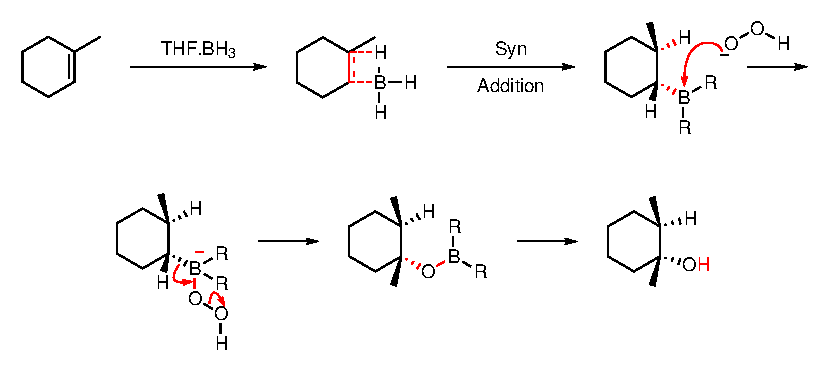
\includegraphics[width=\textwidth]{2-16.eps}
  \end{figure}
  \vspace*{\fill}

\end{landscape}

\subsubsection{Other Alkene Reactions}

\begin{enumerate}[label=\alph*)]

  \item Hydroboration (followed by oxidation) - useful for anti-markovnikov
    hydration.

    \img{2-17}

    Mechanism

    \img{2-18}

    Is electron deficient but commercially available as a complex with the ether
    THF.

    \img{2-19}

    This takes place in a syn addition in a concerted way (both bonds are made
    in the same step). The bond to B is made slightly faster since it is the
    electrophilic center and the electron deficient atom. This results in the
    observed regiochemistry.

    Each of the remaining \ce{B-H} bonds also adds across an alkene to give

    \img{2-21}

    The carbon--boron bond is then replaced by a hydroxyl group with retention
    of configuration.

    \img[The final step occurs via borate ester hydrolysis]{2-22}

\end{enumerate}